\subsection{Question 1}
 Le protocole peut être décrit par le réseau suivant : \\

\begin{comment}
\begin{figure}[H]
  \centering
  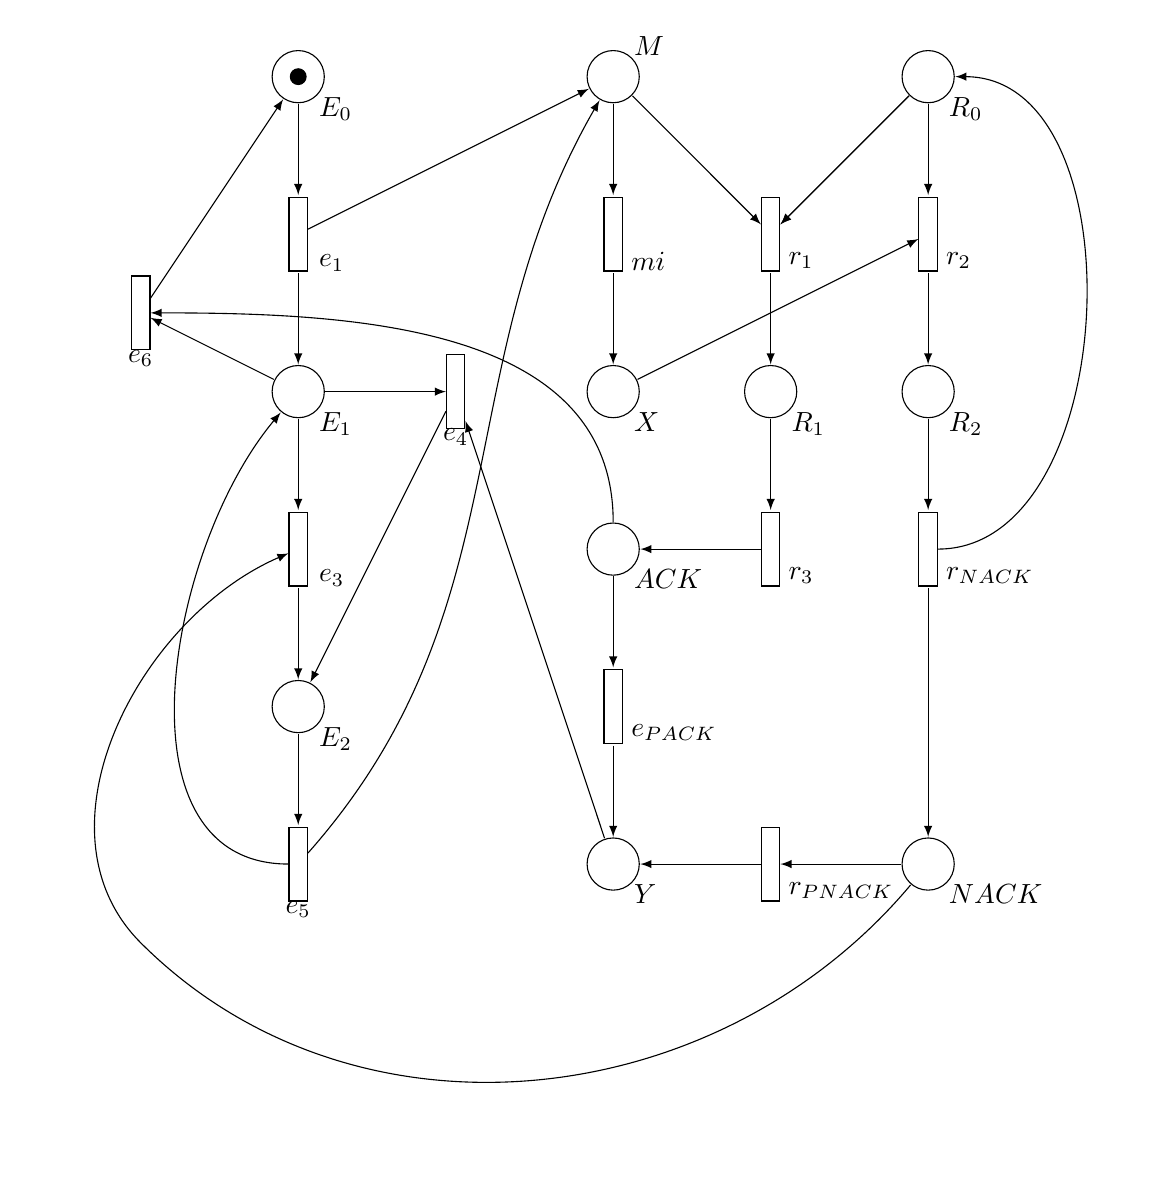
\begin{tikzpicture}
    % Liste des places
    \draw (-4,4) node[below right = 4pt] {$E_0$};
    \node[draw,circle,scale=2] (E0) at (-4, 4) {};
    \draw (-4,0) node[below right = 4pt] {$E_1$};
    \node[draw,circle,scale=2] (E1) at (-4, 0) {};
    \draw (-4,-4) node[below right = 4pt] {$E_2$};
    \node[draw,circle,scale=2] (E2) at (-4, -4) {};
    \draw (0,4) node[above right = 4pt] {$M$};
    \node[draw,circle,scale=2] (M) at (0, 4) {};
    \draw (0,0) node[below right = 4pt] {$X$};
    \node[draw,circle,scale=2] (X) at (0, 0) {};
    \draw (0,-2) node[below right = 4pt] {$ACK$};
    \node[draw,circle,scale=2] (ACK) at (0, -2) {};
    \draw (0,-6) node[below right = 4pt] {$Y$};
    \node[draw,circle,scale=2] (Y) at (0,-6) {};
    \draw (2,0) node[below right = 4pt] {$R_1$};
    \node[draw,circle,scale=2] (R1) at (2, 0) {};
    \draw (4,4) node[below right = 4pt] {$R_0$};
    \node[draw,circle,scale=2] (R0) at (4, 4) {};
    \draw (4,0) node[below right = 4pt] {$R_2$};
    \node[draw,circle,scale=2] (R2) at (4,0) {};
    \draw (4,-6) node[below right = 4pt] {$NACK$};
    \node[draw,circle,scale=2] (NACK) at (4,-6) {};

    % Liste des transitions
    \draw (-6,1) node[below = 10pt] {$e_6$};
    \node[draw,rectangle,yscale=4] (e6) at (-6, 1) {};
    \draw (-4,2) node[below right = 4pt] {$e_1$};
    \node[draw,rectangle,yscale=4] (e1) at (-4, 2) {};
    \draw (-4,-2) node[below right= 4pt] {$e_3$};
    \node[draw,rectangle,yscale=4] (e3) at (-4, -2) {};
    \draw (-4,-6) node[below = 10pt] {$e_5$};
    \node[draw,rectangle,yscale=4] (e5) at (-4, -6) {};
    \draw (-2,0) node[below = 10pt] {$e_4$};
    \node[draw,rectangle,yscale=4] (e4) at (-2, 0) {};
    \draw (0,2) node[below right = 3pt] {$mi$};
    \node[draw,rectangle,yscale=4] (mi) at (0, 2) {};
    \draw (0,-4) node[below right = 3pt] {$e_{PACK}$};
    \node[draw,rectangle,yscale=4] (epa) at (0, -4) {};
    \draw (2,2) node[below right = 3pt] {$r_1$};
    \node[draw,rectangle,yscale=4] (r1) at (2, 2) {};
    \draw (2,-2) node[below right = 3pt] {$r_3$};
    \node[draw,rectangle,yscale=4] (r3) at (2, -2) {};
    \draw (2,-6) node[below right = 3pt] {$r_{PNACK}$};
    \node[draw,rectangle,yscale=4] (rpn) at (2, -6) {};
    \draw (4,2) node[below right = 3pt] {$r_2$};
    \node[draw,rectangle,yscale=4] (r2) at (4, 2) {};
    \draw (4,-2) node[below right = 3pt] {$r_{NACK}$};
    \node[draw,rectangle,yscale=4] (rn) at (4, -2) {};


    % Liste des arcs
    \draw[->,>=latex] (E0) -- (e1);
    \draw[->,>=latex] (e1) -- (E1);
    \draw[->,>=latex] (e1) -- (M);
    \draw[->,>=latex] (E1) -- (e6);
    \draw[->,>=latex] (E1) -- (e4);
    \draw[->,>=latex] (E1) -- (e3);
    \draw[->,>=latex] (M) -- (mi);
    \draw[->,>=latex] (M) -- (r1);
    \draw[->,>=latex] (e6) -- (E0);
    \draw[->,>=latex] (e4) -- (E2);
    \draw[->,>=latex] (e3) -- (E2);
    \draw[->,>=latex] (mi) -- (X);
    \draw[->,>=latex] (r1) -- (R1);
    \draw[->,>=latex] (E2) -- (e5);
    \draw[->,>=latex] (X) -- (r2);
    \draw[->,>=latex] (R1) -- (r3);
    \draw[->,>=latex] (e5) to[out=180,in=230] (E1);
    \draw[->,>=latex] (e5) to[in=240] (M);
    \draw[->,>=latex] (r2) -- (R2);
    \draw[->,>=latex] (r3) -- (ACK);
    \draw[->,>=latex] (R2) -- (rn);
    \draw[->,>=latex] (ACK) -- (epa);
    \draw[->,>=latex] (ACK) to[out=90,in=0] (e6);
    \draw[->,>=latex] (rn) -- (NACK);
    \draw[->,>=latex] (rn) to[out=0,in=0] (R0);
    \draw[->,>=latex] (epa) -- (Y);
    \draw[->,>=latex] (NACK) -- (rpn);
    \draw[->,>=latex] (NACK) to[out=230,in=-45] (-6,-7) to[out=135,in=200] (e3);
    \draw[->,>=latex] (R0) -- (r1);
    \draw[->,>=latex] (R0) -- (r2);
    \draw[->,>=latex] (Y) -- (e4);
    \draw[->,>=latex] (rpn) -- (Y);
    \draw[->,>=latex] (R0) -- (r1);







    % Marquage 
    \draw [fill](-4,4) circle (0.1) ;
  \end{tikzpicture}
  \caption{Réseau de petri associé au protocole de communication} \label{fig:M1}
\end{figure}

\end{comment}

\begin{figure}[H]
  \centering
  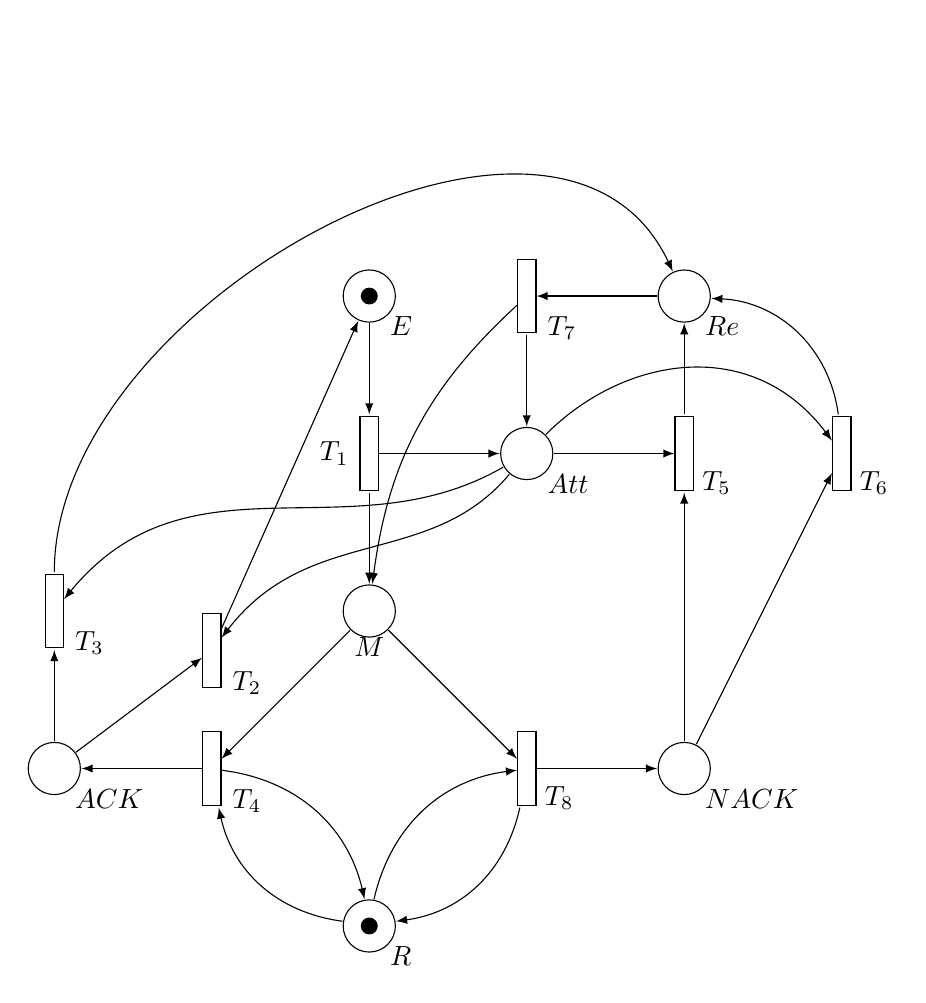
\begin{tikzpicture}
    % Liste des places
    \draw (-2,4) node[below right = 4pt] {$E$};
    \node[draw,circle,scale=2] (E) at (-2, 4) {};
    \draw (-6,-2) node[below right = 4pt] {$ACK$};
    \node[draw,circle,scale=2] (ACK) at (-6, -2) {};
    \draw (-2,0) node[below = 6pt] {$M$};
    \node[draw,circle,scale=2] (M) at (-2,0) {};
    \draw (-2,-4) node[below right = 4pt] {$R$};
    \node[draw,circle,scale=2] (R) at (-2, -4) {};
    \draw (0,2) node[below right = 4pt] {$Att$};
    \node[draw,circle,scale=2] (At) at (0, 2) {};
    \draw (2,4) node[below right = 4pt] {$Re$};
    \node[draw,circle,scale=2] (Re) at (2,4) {};
    \draw (2,-2) node[below right = 4pt] {$NACK$};
    \node[draw,circle,scale=2] (NACK) at (2,-2) {};

    % Liste des transitions
    \draw (-6,0) node[below right= 4pt] {$T_3$};
    \node[draw,rectangle,yscale=4] (T3) at (-6, 0) {};
    \draw (-4,-0.5) node[below right = 4pt] {$T_2$};
    \node[draw,rectangle,yscale=4] (T2) at (-4, -0.5) {};
    \draw (-4,-2) node[below right= 4pt] {$T_4$};
    \node[draw,rectangle,yscale=4] (T4) at (-4, -2) {};
    \draw (-2,2) node[left = 4pt] {$T_1$};
    \node[draw,rectangle,yscale=4] (T1) at (-2, 2) {};
    \draw (0,4) node[below right= 4pt] {$T_7$};
    \node[draw,rectangle,yscale=4] (T7) at (0, 4) {};
    \draw (0,-2) node[below right = 3pt] {$T_8$};
    \node[draw,rectangle,yscale=4] (T8) at (0, -2) {};
    \draw (2,2) node[below right = 3pt] {$T_5$};
    \node[draw,rectangle,yscale=4] (T5) at (2, 2) {};
    \draw (4,2) node[below right = 3pt] {$T_6$};
    \node[draw,rectangle,yscale=4] (T6) at (4, 2) {};


    % Liste des arcs
    \draw[->,>=latex] (E) -- (T1);
    \draw[->,>=latex] (T1) -- (M);
    \draw[->,>=latex] (T1) -- (At);
    \draw[->,>=latex] (M) -- (T4);
    \draw[->,>=latex] (M) -- (T8);
    \draw[->,>=latex] (At) to[out=210,in=45] (T3);
    \draw[->,>=latex] (At) to[out=230,in=45] (T2);
    \draw[->,>=latex] (At) -- (T5);
    \draw[->,>=latex] (At) to[out=45, in=135] (T6);
    \draw[->,>=latex] (T4) -- (ACK);
    \draw[->,>=latex] (T4) to[bend left=35] (R);
    \draw[->,>=latex] (T8) -- (NACK);
    \draw[->,>=latex] (T8) to[bend left=35] (R);
    \draw[->,>=latex] (T3) to[out=90,in=115](Re);
    \draw[->,>=latex] (T2) -- (E);
    \draw[->,>=latex] (T5) -- (Re);
    \draw[->,>=latex] (T6) to[bend right=40] (Re);
    \draw[->,>=latex] (ACK) -- (T3);
    \draw[->,>=latex] (ACK) -- (T2);
    \draw[->,>=latex] (R) to[bend left=35] (T4);
    \draw[->,>=latex] (R) to[bend left=35] (T8);
    \draw[->,>=latex] (NACK) -- (T5);
    \draw[->,>=latex] (NACK) -- (T6);
    \draw[->,>=latex] (Re) -- (T7);
    \draw[->,>=latex] (T7) -- (At);
    \draw[->,>=latex] (T7) to[bend right=20] (M);

    %Marquage
    \draw [fill](-2,4) circle (0.1) ;
    \draw [fill](-2,-4) circle (0.1) ;

  \end{tikzpicture}
  \caption{Réseau de petri associé au protocole de communication} \label{fig:M1}
\end{figure}

\newpage

\subsection{Question 2}

Nous allons représenter le marquagepar un vecteur de la forme :\\
\begin{center}
  (E Att M Re ACK NACK R)\\
\end{center}
où chaque symbole i correspond au nombre de jeton contenu dans la place i.\\
Ainsi $M_0 = (1\ 0\ 0\ 0\ 0\ 0\ 1)$ indique qu'il y a un jeton en E et en R.

\begin{figure}[H]
  \centering
  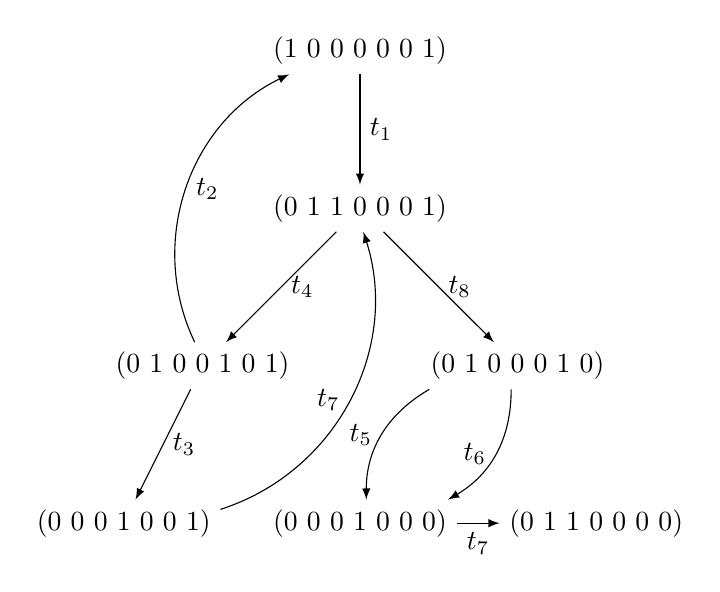
\begin{tikzpicture}
    % Liste des Marquage
    \node (M0) at (0,6) {$(1\ 0\ 0\ 0\ 0\ 0\ 1)$};
    \node (M1) at (0,4) {$(0\ 1\ 1\ 0\ 0\ 0\ 1)$};
    \node (M2) at (-2,2) {$(0\ 1\ 0\ 0\ 1\ 0\ 1)$};
    \node (M3) at (2,2) {$(0\ 1\ 0\ 0\ 0\ 1\ 0)$};
    \node (M4) at (-3,0) {$(0\ 0\ 0\ 1\ 0\ 0\ 1)$};
    \node (M5) at (0,0) {$(0\ 0\ 0\ 1\ 0\ 0\ 0)$};
    \node (M6) at (3,0) {$(0\ 1\ 1\ 0\ 0\ 0\ 0)$};
  

    % Liste des arcs
    \draw[->,>=latex] (M0) -- (M1) node[midway, right]{$t_1$};
    \draw[->,>=latex] (M1) -- (M2) node[midway, right]{$t_4$};
    \draw[->,>=latex] (M1) -- (M3) node[midway, right]{$t_8$};
    \draw[->,>=latex] (M2) to[bend left=45] node[midway, right]{$t_2$} (M0);
    \draw[->,>=latex] (M2) -- (M4) node[midway, right]{$t_3$};
    \draw[->,>=latex] (M3) to[bend right=30] node[midway, left]{$t_5$} (M5);
    \draw[->,>=latex] (M3) to[bend left=30]  node[midway, left]{$t_6$} (M5);
    \draw[->,>=latex] (M4) to[bend right=45] node[midway,left]{$t_7$} (M1);
    \draw[->,>=latex] (M5) -- (M6) node[midway, below]{$t_7$};

  \end{tikzpicture}
  \caption{Graphe des marquages accessibles} \label{fig:M10}
\end{figure}

\subsection{Question 3}

On a dans notre réseau :
\begin{center}
  $a\ =\ T_1\ et\ b\ =\ T_4$
\end{center}

Lors de l'émission d'un message m par l'émetteur, $T_1$ fait transité |m| caractères.\\
On va considérer que l'ensemble du message est reconnu et accepté par le recepteur.\\
Ainsi, $T_4$ fait également transité |m| caractère.\\
Le recepteur envoie alors un ACK et retourne au repos.\\
A ce moment, l'envoie du ACK peut être perturber et transformer en Y. L'emetteur recevant un Y se mat alors en état de réémission et renvoie le message m.\\
Le recepteur le reçoit donc de nouveau.\\
En considerant que le message est reconnu par le recepteur $T_4$ fait à nouveau transité |m| caractère.\\
Le récepteur envoie à nouveau un ACK et nous allons considerer qu'il n'est pas perturber et donc reçu par l'émetteur.\\
Les deux retourne donc à l'état de repos.\\

En notant $w$ la ligne décrite ci-dessus, on a $|T_1|_w = |m|$ et $|T_4|_w = 2|m|$\\
On a donc bien :
\begin{center}
  $|a|_w < |b|_w$
\end{center}


